\documentclass[10pt]{article}
\usepackage[margin=.8in]{geometry}\usepackage{amsmath,amssymb,tikz,hyperref}
\setlength{\parindent}{0pt}\setlength{\parskip}{6pt}
\begin{document}
\textbf{Mumford congruence under affine normalization}\hfill 2026-10-31\\T-1135. Producer formal proof packet; independent source-fidelity review pending.
\section*{Construction}
Over a field $K$, set $T_n(p)=a^{-n}p(aX+b)$. For $a\ne0$ and any natural $d$, the checked transport is
\[u\mid f-v^2\quad\Longrightarrow\quad T_d(u)\mid T_6(f)-T_3(v)^2.\]
When $f-v^2=uq$, the explicit quotient on the right is
\[\frac{a^d}{a^6}\,q(aX+b).\]
Separate declarations check square/difference compatibility, evaluation, root preservation, identity support and zero ordinate.
\begin{center}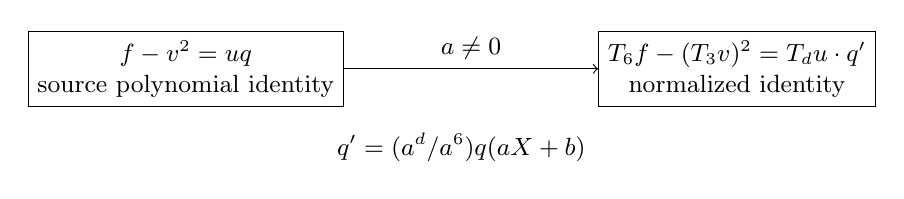
\begin{tikzpicture}[every node/.style={draw,align=center,font=\small}]
\node (a) at (0,0) {$f-v^2=uq$\\source polynomial identity};
\node (b) at (7,0) {$T_6f-(T_3v)^2=T_du\cdot q'$\\normalized identity};
\draw[->] (a)--node[above,draw=none] {$a\ne0$}(b);
\node[draw=none] at (3.5,-1) {$q'=(a^d/a^6)q(aX+b)$};
\end{tikzpicture}\end{center}
\section*{Fixed controls}
Use $f=X^5+1,u=X,v=1,q=X^4,a=2,b=3,d=1$. At the transformed support root $-3/2$, the ordinate is $1/8$ and the curve value is $1/64$. The correct residual is zero. Omitting ordinate scaling yields $-63/64\ne0$. The zero-scale control shows coordinate collapse; that scale is excluded by the main theorem. A fixed divisibility instance is also checked.
\section*{Source connection and remaining bindings}
The historical \texttt{genus2\_model\_gate.rs}, lines14--56, uses these substitution/scaling factors. The preceding Scholten model packet supplies the concrete affine equation. Literal Rust-loop/compiler correspondence, monicity and degree bounds, projective transport and divisor-class interpretation are separate next bindings.
\section*{Evidence}
Nine main declarations and nine controls have separate named axiom readback. Raw attempts, native exit codes, unchanged dependency/source bindings and standardized status accompany this report. Attempt1 failed on polynomial syntax and a looping simplifier; attempt2 corrected them. The first control compile timed out after120 seconds; the identical retry passed. Nonfatal warnings are retained. Existing compiled Lean dependencies remain part of the trust boundary.

Primary documentation: \href{https://leanprover-community.github.io/mathlib4_docs/Mathlib/Algebra/Polynomial/Eval/Defs.html}{Mathlib polynomial evaluation/composition}. No novelty claim. No scientific execution, timing, enumeration or cost ratio; expired campaign limits unchanged. The diagram describes algebraic dependencies, not measured performance.
\end{document}
